\section{TID angewandt 2}
Gehen Sie vom gleichen TID-Konzept wie in Aufgabe \ref{sec:TID_angewandt1} aus.
Die ersten vier Teilaufgaben bauen aufeinander auf.
\sol{Sie können deren Lösung in die leeren Blöcke auf Seite \pageref{fig:TID2_Blocks} eintragen.}

Zu Beginn befindet sich die Datei in folgendem Zustand:

\begin{center}
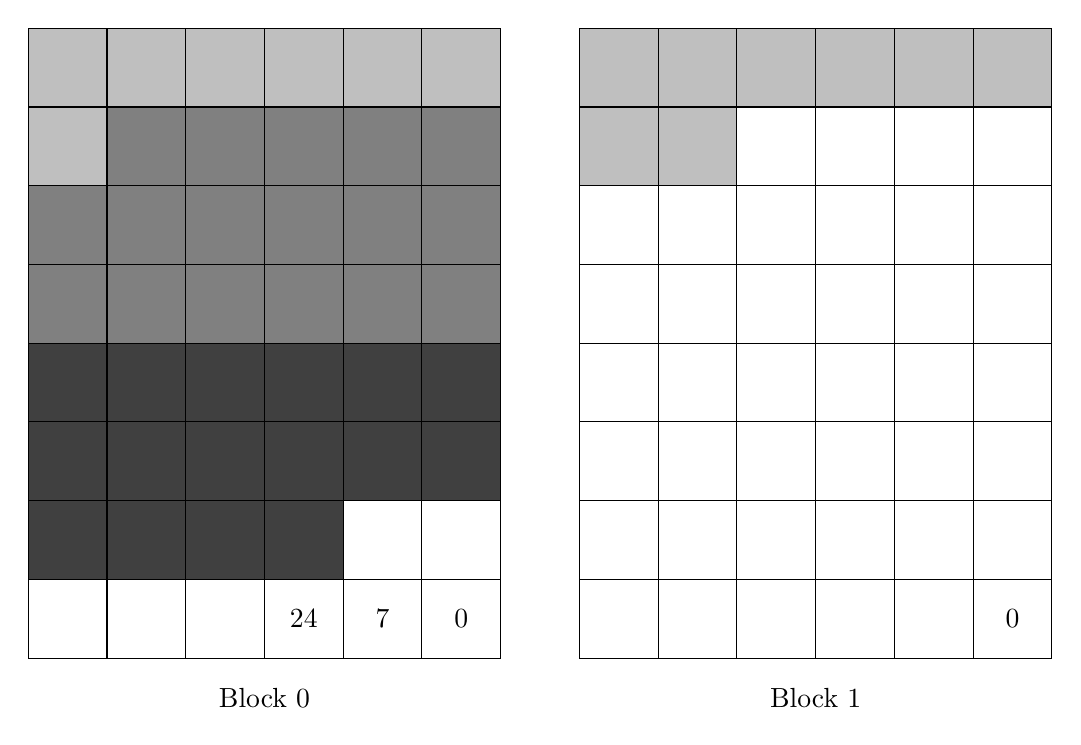
\begin{tikzpicture}
	% Sätze Block 0
	\fill[fill=lightgray] (0,8) rectangle +(6,-2);
	\fill[fill=gray] (1,7) rectangle +(5,-1) (0,6) rectangle +(6,-2);
	\fill[fill=darkgray] (0,4) rectangle +(6,-2) (0,2) rectangle +(4,-1);

	% Sätze Block 1
	\fill[fill=lightgray] (7,8) rectangle +(6,-1) (7,7) rectangle +(2,-1);

	% Index Block 0
	\node at (3.5,0.5) {24};
	\node at (4.5,0.5) {7};
	\node at (5.5,0.5) {0};

	% Index Block 1
	\node at (12.5,0.5) {0};

	% Gitter
	\draw (0,0) grid +(6,8) (7,0) grid +(6,8);

	\node at (3,-0.5) {Block~0};
	\node at (10,-0.5) {Block~1};
\end{tikzpicture}
\end{center}

\begin{normalText}
\begin{enumerate}[a)]
	\item Fügen Sie einen Satz der Größe 12 ein und notieren Sie sich die zugehörige TID.

	\begin{note}
		TID(1,1)
	\end{note}

	\item Vergrößern Sie den Satz mit TID(0,2) auf die Länge 22.
	\item Fügen Sie einen Satz mit Länge 48 ein und notieren Sie sich die zugehörige TID.

	\begin{note}
		TID(2,0)
	\end{note}

	\item Fügen Sie 5 Sätze der Länge 2 ein und notieren Sie sich die zugehörigen TIDs. Was fällt Ihnen hierbei auf?

	\begin{note}
		TID(0,4), TID(0,5), TID(0,6), TID(0,7), TID(0,8)

		Kleine Sätze verbrauchen viel Speicher für die Organisation.
	\end{note}

\begin{solution}
\begin{figure}
\begin{tikzpicture}
	\begin{note}
		% Sätze Block 0
		\fill[fill=blue!25] (0,17) rectangle +(6,-2);
		\fill[fill=blue!40] (1,16) rectangle +(5,-1) (0,15) rectangle +(6,-2);
		%b)
		\fill[fill=blue!50] (0,13) rectangle +(2,-1);
		%c)
		\filldraw[fill=blue!75] (2,13) rectangle + (3,-1);
		%d)
		\filldraw[fill=blue!20] (5,13) rectangle + (1,-1); %1
		\filldraw[fill=blue!20] (0,12) rectangle + (1,-1);
		\filldraw[fill=blue!60] (1,12) rectangle + (2,-1); %2
		\filldraw[fill=blue!30] (3,12) rectangle + (2,-1); %3
		\filldraw[fill=blue!70] (5,12) rectangle + (1,-1); %4
		\filldraw[fill=blue!70] (0,11) rectangle + (1,-1);
		\filldraw[fill=blue!40] (1,11) rectangle + (2,-1); %5


		% Sätze Block 1
		\fill[fill=blue!75] (7,17) rectangle +(6,-1) (7,16) rectangle +(2,-1);
		%a)
		\fill[fill=blue!25] (9,16) rectangle + (4,-1) (7,15) rectangle +(6,-1) (7,14) rectangle +(2,-1);
		%b)
		\fill[fill=blue!50] (9,14) rectangle +(4,-1) (7,13) rectangle +(6,-3);

		% Sätze Block 2
		%c)
		\fill[fill=blue!75!black] (0, 8) rectangle +(2, -1);
		\fill[fill=blue!75] (2,8) rectangle +(4, -1) (0, 7) rectangle +(6, -6) (0, 1) rectangle +(5, -1);
		% Index Block 0
		\node at (3.5,9.5) {24};
		\node at (4.5,9.5) {7};
		\node at (5.5,9.5) {0};
		%b)
		\node at (1,12.5) {TID(1,2)};
		%c)
		\node at (2.5, 9.5) {26};
		%d)
		\node at (1.5,9.5) {29}; %1
		\node at (0.5,9.5) {31}; %2
		\node at (5.5,10.5) {33}; %3
		\node at (4.5,10.5) {35}; %4
		\node at (3.5,10.5) {37}; %5
		% Index Block 1
		\node at (12.5,9.5) {0};
		%a)
		\node at (11.5,9.5){8};
		%b)
		\node at (10.5,9.5){20};

		%Index Block 2
		\node at (5.5, 0.5) {0};
		\node at (1,7.5) {\color{white}TID(0, 3)};
	\end{note}

	% Gitter
	\draw (0,0) grid +(6,8) (7,0) grid +(6,8) ;
	\draw (0,9) grid +(6,8) (7,9) grid +(6,8);
	\node at (3,8.5) {Block~0};
	\node at (10,8.5) {Block~1};
	\node at (3,-0.5) {Block~2};
	\node at (10,-0.5) {Block~3};
\end{tikzpicture}
\label{fig:TID2_Blocks}
\end{figure}
\end{solution}
\pagebreak

	\item Löschen Sie nun aus der folgenden Skizze den Satz mit TID(0,1).
	\begin{center}
		\begin{tikzpicture}
		% Sätze Block 0 Vorher
		\fill[fill=lightgray] (0,8) rectangle +(6,-2);
		\fill[fill=gray] (1,7) rectangle +(5,-1) (0,6) rectangle +(6,-2);
		\fill[fill=darkgray] (0,4) rectangle +(6,-2) (0,2) rectangle +(4,-1);

		% Index Block 0 Vorher
		\node at (3.5,0.5) {24};
		\node at (4.5,0.5) {7};
		\node at (5.5,0.5) {0};
		\begin{note}
		% Sätze Block 0 Nachher
		\fill[fill=blue!25] (7,8)  rectangle +(6,-2);
		\fill[fill=blue!50] (8,7) rectangle +(5,-1) (7,6) rectangle +(6,-1) (7,5) rectangle +(5,-1) ;

		% Index Block 0 Nachher
		\node at (12.5,0.5) {0};
		\node at (11.5,0.5) {/};
		\node at (10.5,0.5) {7};
		\end{note}
		% Gitter
		\draw (0,0) grid +(6,8) (7,0) grid +(6,8);

		\node at (3,-0.5) {Block~0~Vorher};
		\node at (10,-0.5) {Block~0~Nachher};


		\end{tikzpicture}
	\end{center}

	\begin{note}
		Hinweis: Es ist vermutlich implementierungsabhängig, ob Block~0 gleich reorganisiert wird, d.h. ob TID(0, 2) nach vorne geschoben wird.
	\end{note}
\end{enumerate}
\end{normalText}
